\subsection{Flyvehøjde}

Dette afsnit beskriver test af tilpasning af flyvehøjde.

For at dronen ved hvilken højde den skal flyve i, skal flyveopsætningen være hentet fra serveren. Når flyvehøjden og de ønskede GPS positioner er kendt, begynder dronen at lette. Main controlleren anvender højdesensorer til at finde højden med. Så længe at højden ikke er indenfor det ønskede interval, skal den hæve eller sænke sin højde, det gør den ved enten at forøge eller formindske throttle. 

På figur \ref{fig:skift_hoejde} ses hvad der sker, hvis højden enten er for høj eller for lav. Først måles den aktuelle højde, denne sammenlignes med minimumshøjden og den maksimalehøjde, hvis den er udenfor det interval reguleres der på throttle. 

\begin{figure}[H]
\centering
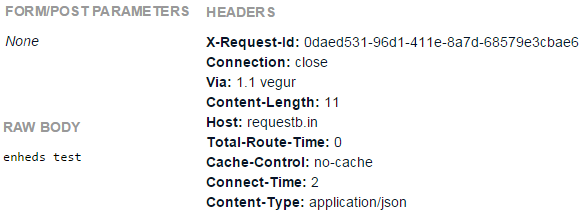
\includegraphics[width=0.8\textwidth]{Billeder/Test/put_request.png}
\caption{Tilpasning af højde}
\label{fig:skift_hoejde}
\end{figure}